%
% 5-homologie.tex
%
% (c) 2026 Prof Dr Andreas Müller
%
\section{Homologie
\label{buch:integration:section:homologie}}
\kopfrechts{Homologie}%
In Anwendungen des cauchyschen Integralsatzes kommt es auf die Wahl
eines geeigneten Weges an.
Schon im Beweis des Integralsatzes wurde das Argument verwendet, dass
Wegestücke, die zweimal in entgegengesetzter Richtung durchlaufen
werden, keinen Betrag zum Integral leisten.
Ein beliebiger Weg, der einmal den Punkt $z_0$ umläuft, führt auf die
gleichen Werte des Integrals wie ein kleiner Kreis um den Punkt $z_0$.
Es scheint also gar nicht so sehr auf den Verlauf des Weges anzukommen,
sondern nur darauf, was wie oft umlaufen wird.
Der Begriff der \emph{Homologie} versucht diese Beobachtung
zu präzisieren.

%
% 51-kettenzyklen.tex -- Ketten und Zyklen
%
% (c) 2026 Prof Dr Andreas Müller
%
\subsection{Ketten und Zyklen}
Der Integralsatz von Cauchy besagt, dass ein Deformation des Weges
eines Wegintegrals sich nicht auf den Wert des Integrals auswirkt,
solange die Deformation keine Singulartität der Funktion trifft.
%
% fig-paar.tex
%
% (c) 2026 Prof Dr Andreas Müller
%
\begin{figure}
\centering
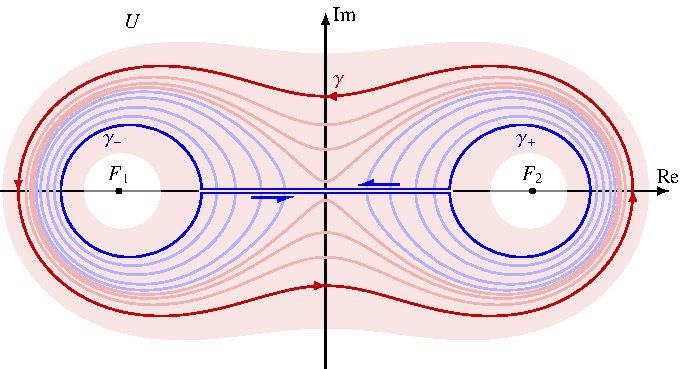
\includegraphics{chapters/030-integration/images/paar.pdf}
\caption{Deformation des Weges $\gamma$ in einen Weg, der die
beiden ``Löcher'' jeweils einmal umlaufen.
Die beiden Wegteile entlang der reellen Achse werden in
entgegengesetzter Richtung durchlaufen, die zugehörigen
Integrale heben sich daher weg.
Der Weg $\gamma$ ist \emph{homolog} zur Summe der Wegen
$\gamma_+$ und $\gamma_-$.
\label{buch:integration:homologie:fig:paar}}
\end{figure}
%
Abbildung~\ref{buch:integration:homologie:fig:paar}
zeigt die Deformation des Pfades $\gamma$, der die beiden ``Löcher''
im Definitionsbereich um die Foki $F_1$ und $F_2$ der Lemniskate
einmal umläuft, in zwei Wege $\gamma_+$ und $\gamma_-$, die $F_1$
und $F_2$ separat umlaufen, verbunden über zwei Wegstücke entlang
der reellen Achse, die in entgegengesetzter Richtung durchlaufen
werden und sich im Integral daher wegheben.
Es folgt, dass
\[
\int_\gamma f(z)\,dz
=
\int_{\gamma_+} f(z)\,dz
+
\int_{\gamma_-} f(z)\,dz.
\]
Wir müssen daher die Idee eines Weges wie $\gamma$ zu einer 
Vereinigung von Wegen wie $\{\gamma_+,\gamma_-\}$ verallgemeinern.

\begin{definition}[Kette]
\label{buch:integration:homologie:def:kette}
Eine \emph{Kette} $C$ in $U$ ist eine formale Summe
\index{Kette}%
\begin{equation}
c
=
c_1\gamma_1 + \dots + c_n\gamma_n
\label{buch:integration:homologie:eqn:def:kette}
\end{equation}
von Wegen $\gamma_k\colon I \to U$ mit $c_k\in\mathbb{Z}$.
Wir bezeichnen mit
\[
C_1
=
C_1
=
\{
c_1\gamma_1+\ldots+c_n\gamma_n
\mid
\gamma_k:I\colon U, c_k\in \mathbb{Z}
\}
\]
die Menge der (eindimensionalen) Ketten.
\end{definition}

Die Definition unterscheidet alle Wege, auch solche, die ineinander
deformierbar sind.
%
% fig-kettenzyklen.tex
%
% (c) 2026 Prof Dr Andreas Müller
%
\begin{figure}
\centering
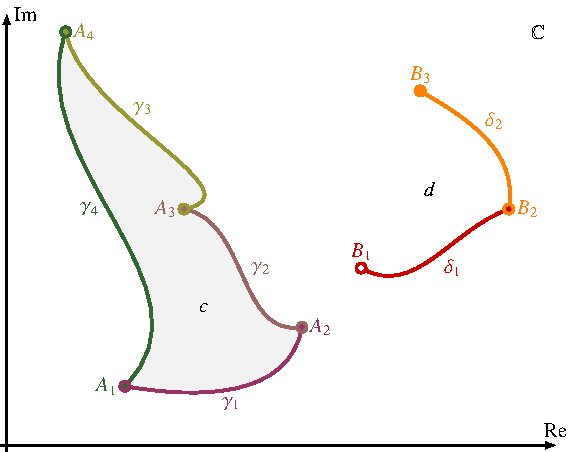
\includegraphics{chapters/030-integration/images/kettenzyklen.pdf}
\caption{Ketten $c=\gamma_1+\gamma_2+\gamma_3+\gamma_4$ und
$d=\delta_1+\delta_2$ sind Linearkombinationen von Wegen.
Der Randoperator extrahiert die Endpunkte mit einem Vorzeichen.
Anfangspunkte sind also offene Kreise, Endpuntke als ausgefüllte
Kreise dargestellt.
Für die Kette $d$ ist $\partial d = B_3-B_1$.
Für die Kette $c$ kommt in $\partial c$ jeder Punkt mit positivem
und negativem Vorzeichen vor, es ist $\partial c=0$.
\label{buch:integration:homologie:fig:kettenzyklen}}
\end{figure}
%
Es wird auch nicht verlangt, dass die Wege geschlossen sind.
Die Wege können geschlossen sein, es kann aber auch sein, dass sich
die Wege zu einem geschlossenen Weg zusammensetzen lassen.

\begin{definition}[Randoperator]
\label{buch:integration:homologie:definition:randoperator}
Die Menge der \emph{$0$-dimensionalen Ketten} ist
\index{Ketten!0-dimensional}%
\[
C_0 
=
C_0(U)
=
\{
c_1P_1+\ldots+c_nP_n
\mid
c_k\in \mathbb{Z}, P_k\in U
\}.
\]
Sie besteht aus formalen Linearkombinationen von Punkten in $U$.
Der \emph{Randoperator} ist eine
\index{Randoperator}%
lineare Abbildung $\partial \colon C_1\to C_0$, die einen
Weg $\gamma$ auf
\[
\gamma \mapsto 1\cdot \gamma(1) - 1\cdot \gamma(0)
\]
abbildet.
\end{definition}

Der Endpunkt eines Weges erhält also das Gewicht $1$, während der
Anfangspunkt das Gewicht $-1$ erhält.
Mehrere Wege können zusammengesetzt werden, wenn der Endpunkt
eines Wegestückes mit den Anfangspunkt des nächsten Stücks
übereinstimmt, wenn also $\gamma_k(1) = \gamma_{k+1}(0)$ gilt.
Der Randoperator bildet $\gamma_k + \gamma_{k+1}$ auf
\[
\partial ( \gamma_k + \gamma_{k+1} )
=
-\gamma_k(0) + \gamma_k(1) -\gamma_{k+1}(0) + \gamma_{k+1}(1)
=
-\gamma_k(0) + \gamma_{k+1}(1)
\]
ab.
Die Zusammensetzbarkeit der Wege ist also genau dann gegeben, 
wenn sich bei Anwendung des Randoperators die Punkte, wo die
Wege zusammengesetzt werden müssen, wegheben.
In Abbildung~\ref{buch:integration:homologie:fig:kettenzyklen}
tritt diese Situation im Zyklus $d$ beim Punkt $B_2$ ein.
Wenn sich alle Punkte wegheben, dann lassen sich die Wegstücke
zu einem geschlossenen Weg zusammensetzen.
In Abbildung~\ref{buch:integration:homologie:fig:kettenzyklen}
tritt dies für den Zyklus $c$ ein.
Wir definieren daher einen Zyklus wie folgt.

\begin{definition}[Zyklus]
\label{buch:integration:homologie:definition:zyklus}
Ein \emph{Zyklus} ist eine Kette in $C_1$, deren Rand verschwindet:
\index{Zyklus}%
\[
Z_1
=
Z_1(U)
=
\{
c\in C_1
\mid
\partial c = 0
\}.
\]
\end{definition}

In Abbildung~\ref{buch:integration:homologie:fig:kettenzyklen} sind
zwei Ketten $c=\gamma_1+\gamma_2+\gamma_3+\gamma_4$ und $d=\delta_1+\delta_2$
dargestellt.
Der Randoperator von $d$ ist
\begin{align*}
\partial d
&=
\partial\delta_1
+
\partial\delta_2
=
B_2-B_1 + B_3-B_2
=
B_3-B_1,
\intertext{es bleiben also die Puntke $B_3$ und $B_1$ mit verschiedenen
Vorzeichen.
Für $c$ ist der Randoperator}
\partial c
&=
\partial \gamma_1
+
\partial \gamma_2
+
\partial \gamma_3
+
\partial \gamma_4
=
A_2-A_1
+
A_3-A_2
+
A_4-A_3
+
A_1-A_4
=
0,
\end{align*}
die Kette $c$ ist also ein Zyklus.
Jeder Teilweg beginnt im Endpunkt eines anderen Weges und endet
im Anfangspunkt eines anderen Weges.

%
% 52-kettenintegral.tex -- Integral über Ketten
%
% (c) 2026 Prof Dr Andreas Müller
%
\subsection{Integral über Ketten}
Damit das Wegintegral eine lineare Abbildung von Ketten wird, 
muss das Wegintegral entlang einer Kette durch Linearkombination
der einzelnen Integrale gebildet werden:

\begin{definition}[Wegintegral einer Kette]
Ist $c\in C_1$ eine Kette der Form
\eqref{buch:integration:homologie:eqn:def:kette}
und $f$ eine in $U$ holomorphe Funktion, dann ist das 
\emph{Wegintegral entlang $C$} definiert durch
\index{Wegintegral entlang einer Kette}%
\index{Kettenintegral}%
\begin{equation}
\int_c f(z)\,dz
=
c_1
\int_{\gamma_1}f(z)\,dz
+
\ldots
+
c_n
\int_{\gamma_n}f(z)\,dz
=
\sum_{k=1}^n
c_k \int_{\gamma_k} f(z)\,dz.
\label{buch:integration:homologie:eqn:kettenintegral}
\end{equation}
\end{definition}

Ist $F(z)$ eine Stammfunktion von $f(z)$, dann kann das Integral über
die Komponenten $\gamma_k$ der Kette ausgerechnet werden und es
gilt
\[
\int_c f(z)\,dz
=
\sum_{k=1}^n c_k \int_{\gamma_k}f(z)\,dz
=
\sum_{k=1}^n c_k
\Bigl[F(z)\Bigr]_{\gamma_k(0)}^{\gamma_k(1)}
=
\sum_{k=1}^n c_k
\bigl(
F(\gamma_k(1)) - F(\gamma_k(0))
\bigr)
\]
Die Klammer im letzten Term kann man interpretieren als die
Auswertung der Funktion $F$ auf dem Rand des Wegstückes $\gamma_k$.
Schreibt man dies rein formal als das Integral
\[
\int_{\partial\gamma_k} F(z)\,dz
=
\Bigl[
F(z)
\Bigr]_{\gamma_k(0)}^{\gamma_k(1)},
\]
dann kann man die Gleichung
\eqref{buch:integration:homologie:eqn:kettenintegral}
als
\begin{equation}
\int_{\partial c} F(z)\,dz
=
\int_c F'(z)\,dz
\label{buch:integration:homologie:eqn:stokes0}
\end{equation}
schreiben.
Diese Formel ist ein Beispiel für den allgemeinen Satz von Stokes
\index{Satz!von Stokes}%
aus der Theorie der Differentialformen.
\index{Differentialform}
Er besagt, dass das Integral der Ableitung einer Differentialform
über ein Gebiet ersetzt werden kann durch das Integral der Differentialform
über den Rand.
In der Schreibweise der Differentialformen wird dies für eine
Differentialform $\omega$ und das Gebiet $S$ als
\[
\int_{\partial S}\omega
=
\int_S d\omega
\]
geschrieben, $d\omega$ ist die äussere Ableitung der Differentialform.
Die Ähnlichkeit mit
\eqref{buch:integration:homologie:eqn:stokes0}
ist unverkennbar.

%
% Integral über Zyklen
%
\subsubsection{Integral über Zyklen}
Ist $c$ ein Zyklus, dann lassen sich die Teilwege von $c$ zu einem
geschlossenen Weg zusammen setzen, wie dies in
Abbildung~\ref{buch:integration:homologie:fig:kettenzyklen}
dargestellt ist.
In diesem Fall ist es sinnvoll vom Integral über einen geschlossen
Weg zu sprechen und
\[
\partial c = 0
\qquad\Rightarrow\qquad
\int_c f(z)\,dz
=
\oint_c f(z)\,dz
\]
zu schreiben.

Abbildung~\ref{buch:integration:homologie:fig:paar}
zeigt eine Situation einer Kette $C=\gamma_++\gamma_-$, deren
Wegintegral
\[
\int_C f(z)\,dz
=
\int_{\gamma_+} f(z)\,dz
+
\int_{\gamma_-} f(z)\,dz
=
\int_{\gamma} f(z)\,dz
\]
mit dem Wegintegral entlang der Kurve $\gamma$ übereinstimmt.
Soweit es um Wegintegrale entlang einer Kette geht, gibt es 
zwischen $\gamma$ und $C$ keinen Unterschied.

Zwischen $\gamma$ und nur der Komponente $\gamma_+$ gibt es
ein wesentlichen Unterschied.
Die Funktion $f(z) = 1/(z-F_1)$ hat eine Polstelle im Punkt $F_1$.
Die Wegintegrale
\begin{align*}
\frac{1}{2\pi i}
\oint_\gamma f(z)\,dz
&=
\\
\frac{1}{2\pi i}
\oint_\gamma \frac{1}{z-F_1}\,dz
&=
\\
\operatorname{ind}_\gamma(F_1)
&=
1
\\
&\ne
\frac{1}{2\pi i}
\oint_{\gamma_+} f(z)\,dz
\\
&=
\frac{1}{2\pi i}
\oint_{\gamma_+} \frac{1}{z-F_1}\,dz
\\
&=
\operatorname{ind}_{\gamma_+}(F_1)
\\
&=
0
\end{align*}
sind jedoch verschieden.
Der Grund dafür ist, dass $\gamma$ und $\gamma_+$ den Punkt $F_1$
nicht gleich oft umlaufen.
Wir definieren daher ein Äquivalenzrelation von Ketten durch die
Anzahl der Male, die sie Punkte ausserhalb von $U$ umlaufen.

\begin{definition}[Umlaufzahl einer Kette]
Die \emph{Umlaufzahl} einer Kette $C$ um einen Punkt $z_0$ ist
\index{Umlaufzahl}%
\[
\operatorname{ind}_C(z_0)
=
\frac{1}{2\pi i}
\int_C
\frac{1}{z-z_0}
\,dz.
\]
\end{definition}

%
% 53-homologie.tex -- Homologie von Ketten
%
% (c) 2026 Prof Dr Andreas Müller
%
\subsection{Homologie von Ketten
\label{buch:integration:homologie:subsection:homologie}}
Die Homotpieeigenschaft des Wegintegrals hat gezeigt, dass sich der
Wert eines Wegintegrals einer holomorphen Funktion nicht ändert, wenn
man den Weg stetig deformiert.
Dies wurde zum Beispiel in
Abbildung~\ref{buch:integration:homologie:fig:residuum}
verwendet, um zu zeigen, dass der Weg $\gamma$ und der kleine Kreis
um den Punkt $z_0$ zu den gleichen Werten der Wegintegrale führen.
Diese Äquivalenz von Ketten, die zu gleichen Wegintegralen führen,
verdient einen eigenen Namen.

\begin{definition}[homolog]
Die geschlossene Ketten $c_1$ und $c_2$ heissen \emph{homolog} in $U$,
in Zeichen $c_1\sim c_2$ oder $c_1\sim_{U}c_2$, wenn
\index{homolog}%
für jeden Punkt $a\in \mathbb{C}\setminus U$ ausserhalb von $U$
die Umlaufzahlen
\[
\operatorname{ind}_{c_1}(a)
=
\operatorname{ind}_{c_2}(a)
\]
von $c_1$ und $c_2$ um $a$ gleich sind.
\end{definition}

Die Kette $\gamma_++\gamma_-$ in
Abbildung~\ref{buch:integration:homologie:fig:paar} ist zu $\gamma$ homolog,
da beide Ketten jedes der Löcher $F_1$ und $F_2$ genau einmal umrunden.
Für homologe Ketten ist nicht nur die Umlaufzahl gleich, sondern
jedes Integral einer holomorphen Funktion über die Ketten.

\begin{satz}
\label{buch:integration:homologie:satz:cauchyketten}
Sei $U$ ein Gebiet in $\mathbb{C}$ und
$c$ eine Kette, die homolog zu $0$ ist.
Dann ist
\[
\int_c f(z)\,dz = 0
\]
für jede in $U$ holomorphe Funktion.
\end{satz}

Aus diesem Satz folgt sofort das folgende Korollar.
Es zeigt, dass es bei Kettenintegralen von holomorphen Funktionen
nur auf die Homologieklasse der Kette ankommt, über die integriert
wird.
Sind Ketten homolog, ergibt sich auch der gleiche Wert des Integrals.

\begin{korollar}
Sind die Ketten $c_1$ und $c_2$ homolog, dann ist
\[
\int_{c_1} f(z)\,dz
=
\int_{c_2} f(z)\,dz.
\]
\end{korollar}

\begin{proof}
Die Kette $c=c_1-c_2$ ist homolog zu 0 und daher
\[
0
=
\int_c f(z)\,dz
=
\int_{c_1}f(z)\,dz - \int_{c_2}f(z)\,dz
\qquad\Rightarrow\qquad
\int_{c_1}f(z)\,dz = \int_{c_2}f(z)\,dz.
\qedhere
\]
\end{proof}

Der Satz~\ref{buch:integration:homologie:satz:cauchyketten}
macht keine Voraussetzung weiteren Voraussetzungen an die Funktion
als dass sie in $U$ holomorph sein muss.
Die Funktionen $z\mapsto 1/(z-z_0)$ mit $z_0\in\mathbb{C}\setminus U$
sind alle holomorph in $U$.
Die Integrale über die Kette ergeben die Umlaufzahlen.
Da die Ketten 0-homolog sind, müssen alle diese Umlaufzahlen 0
ergeben.

Für beliebige Funktionen $f(z)$ können wir in der Umgebung eines
Punktes immer eine lokale Stammfunktion finden, die ausserdem
unabhängig ist vom Weg.
Zum Beispiel wissen wir schon, dass Wegintegrale über den Rand
von Rechtecke immer verschwinden, wenn $f(z)$ holomorph ist im
ganzen Rechteck.
Auch wissen wir dies bereits für geschlossene und zusammenziehbare
Wege.
Die Hauptaufgabe des Beweises ist also, diese Erkenntnisse auf 
Ketten zu verallgemeinern, die weit auseinanderliegende Komponenten
haben können.

Um den Satz zu beweisen, verfolgen wir die folgende Strategie.
\begin{enumerate}
\item
Zunächst approximieren wir die Kette durch eine Kette, deren
Wege alle aus achsenparallelen Segmenten bestehen.
Die Kettenintegrale ändern sich dadurch nicht.
\item
Wir zerlegen den achsenparallelen Weg in eine Summe von Rändern
von Rechtecken, die vollständig in $U$ enthalten sind.
\item 
Wir berechnen das Integral über die Kette als Summe über die Integrale
über die Ränder der Rechtecke.
\end{enumerate}

%
% fig-treppe.tex
%
% (c) 2026 Prof Dr Andreas Müller
%
\begin{figure}
\centering
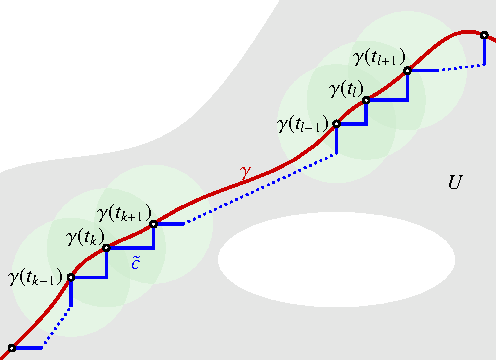
\includegraphics{chapters/030-integration/images/treppe.pdf}
\caption{Approximation eines Weges $\gamma$ in einer Kette durch eine Kette
von achsenparallelen Segmenten $\tilde{c}$.
\label{buch:integration:fig:treppe}}
\end{figure}
%

%
% fig-gitterapprox.tex -- Beweis des Homologie-Satzes
%
% (c) 2026 Prof Dr Andreas Müller
%
\begin{figure}
\centering
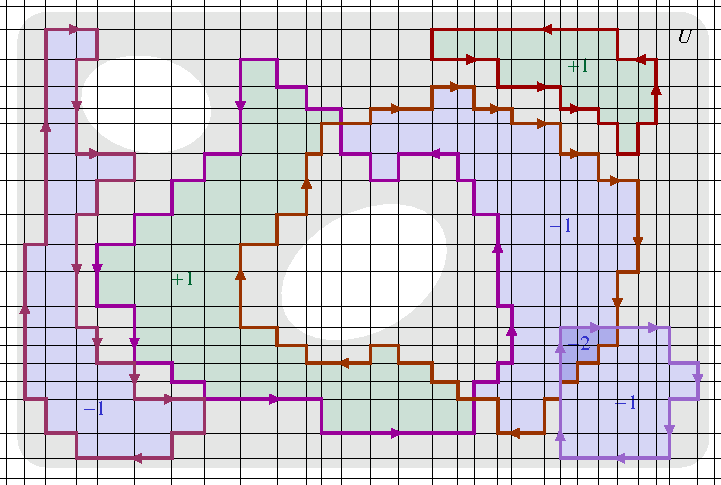
\includegraphics{chapters/030-integration/images/gitterapprox.pdf}
\caption{Eine nullhomologe Kette lässt sich durch eine nullhomologen Kette
$c$ mit achsparallelen Segmenten approximieren, ohne dass sich
Integrale ändern.
Die Segmente definieren eine Unterteilung der Ebene in Rechtecke.
Jedem Rechteck $R_i$ wird die Umlaufzahl $m_i=\operatorname{ind}_{c}(a_i)$
eines Punktes $a_i\in R_i$ zugeordnet.
Die farbigen Rechtecke haben $m_i\ne 0$.
Die Kette ist $c=\sum_i m_i\partial R_i$.
\label{buch:integration:fig:gitterapprox}}
\end{figure}
%

\begin{proof}[Beweis von Satz~\ref{buch:integration:homologie:satz:cauchyketten}]
\begin{enumerate}
\item
Approximation des Weges $\gamma$.

Die Kette $c$ besteht aus einzelnen differenzierbaren Wegen $\gamma$.
Mit jedem Punkt einer Kurve ist auch eine genügend kleine Kreisscheibe
um den Punkt in $U$ enthalten (Abbildung~\ref{buch:integration:fig:treppe}).
Da die Kurve kompakt ist, kann man sie mit endlich vielen solchen Kreisen
abdecken.
In jeder Kreisscheibe kann man auf dem Weg Punkte auswählen, so dass 
zu jeweils zwei aufeinanderfolgenden Punkten auf dem Weg auch das von
den Punkte aufgespannte Rechteck in $U$ ist.
Der Weg kann also durch Teile des Randes dieser Rechtecke ersetzt werden.
Die Umlaufzahlen und Integrale ändern sich dabei nicht, da die 
Rechtecke so klein sind, dass das die Funktionen eine Stammfunktion haben.
Wir ersetzen die Ketten durch eine Kette bestehend aus diesen Randsegmenten.

\item
Aufteilung der Ebene in Rechtecke.

Wir zerlegen die komplexe Ebene durch achsparallele Geraden durch
alle Eckpunkte, die bei der Unterteilung der Kette gefunden wurden
(Abbildung~\ref{buch:integration:fig:gitterapprox}).
Dadurch werden einige der achsparallelen Segmente weiter unterteilt.
Wir bezeichnen die Rechtecke mit $R_i$ und ersetzen die Kette
durch Randsegmente dieser Rechecke.

\item
Selektion der Rechtecke.

In jedem Rechteck wählen wir einen Punkt $\alpha_i\in R_i$ und berechnen
die Umlaufzahl $m_i=\operatorname{ind}_\gamma(\alpha_i)$.
Die Umlaufzahl ist im Inneren jedes Rechtecks konstant.
Wenn $m_i\ne 0$ ist, dann muss $R_i\in U$ sein, denn Punkte ausserhalb
von $U$ würden eine Umlaufzahl $0$ geben, weil $c$ nullhomolog ist.

\item $\displaystyle c=\sum_i m_i\partial R_i$.

%
% fig-nachbar.tex
%
% (c) 2026 Prof Dr Andreas Müller
%
\begin{figure}
\centering
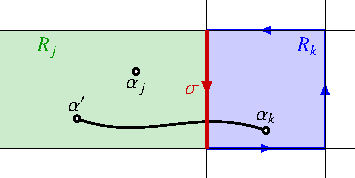
\includegraphics{chapters/030-integration/images/nachbar.pdf}
\caption{Fehlerhafte Kante $\sigma$ des Rechtecks $R_k$ mit Nachbarrechteck $R_j$
für den letzten Schritt des Beweises von Satz
\ref{buch:integration:homologie:satz:cauchyketten}.
\label{buch:integration:fig:nachbar}}
\end{figure}


Angenommen, eine Kante $\sigma$ eines der Rechtecke ist nicht mit der korrekten
Anzahl in $c$ (Abbildung~\ref{buch:integration:fig:nachbar}).
Sei $R_k$ dieses Rechteck.
Dann gibt es eine ganze Zahl $m$ derart, dass
\[
C
=
c-\sum_i m_i\partial R_i - m\partial R_k
\]
die Kante nicht mehr enthält.
Sei $R_j$ das ebenfalls an die Kante $\sigma$ angrenzende Rechteck und
$\alpha'$ ein Punkt in diesem Rechteck.
Da $\sigma$ in $C$ nicht mehr vorkommt, kann man einen Punkt stetig von $\alpha_k$
nach $\alpha'$ verschieben, ohne $C$ zu kreuzen.
Die Umlaufzahl von $C$ kann sich dabei nicht ändern, also muss $C$ gleiche
Umlaufzahlen um  $\alpha_k$ und $\alpha'$ haben.
Andererseits ist die Umlaufzahl linear, d.~h. 
\begin{align*}
\operatorname{ind}_C(\alpha_k)
&=
\operatorname{ind}_{c-\sum_i m_i\partial R_i - m\partial R_k}(\alpha_k)
\\
&=
\operatorname{ind}_c(\alpha_k)
-
\sum_i m_i\operatorname{ind}_{\partial R_i}(\alpha_k)
-
m\operatorname{ind}_{\partial R_k}(\alpha_k)
\\
&=
\operatorname{ind}_c(\alpha_k)
-
\sum_i m_i\delta_{ik}
-
m.
\intertext{Der erste Term ist nach der Definition der Zahlen $m_i$}
&= m_k - m_k - m.
\end{align*}
Andererseits ist $\operatorname{ind}_C(\alpha')$ zu bestimmen.
Falls $\alpha'$ in einem unendlichen Rechteck liegt, ist 
$\operatorname{ind}_C(\alpha')=0$.
Falls $R_j$ ein endliches Rechteck ist, dann ist
$\operatorname{ind}_{c}(\alpha')=\operatorname{ind}_c(\alpha_j)$
und es folgt
\begin{align*}
\operatorname{ind}_C(\alpha')
&=
\operatorname{ind}_{c-\sum_i m_i\partial R_i - m\partial R_k}(\alpha_j)
\\
&=
\operatorname{ind}_{c}(\alpha_j)
-
\sum_i m_i\operatorname{ind}_{\partial R_i}(\alpha_j)
-
m\operatorname{ind}_{\partial R_k}(\alpha_j)
\\
&=
m_j - \sum_i m_i\delta_{ij}
=
m_j-m_j 0 0.
\end{align*}
In beiden Fällen ist $\operatorname{ind}_C(\alpha')=0$ und es folgt,
dass $m=0$, d.~h.~$\sigma$ kam in der Kette gar nicht mit der falschen
Anzahl vor.
\qedhere
\end{enumerate}
\end{proof}

Wir betrachten jetzt einen später besonders nützlichen Spezialfall.
%
% fig-merohomolog.tex
%
% (c) 2026 Prof Dr Andreas Müller
%
\begin{figure}
\centering
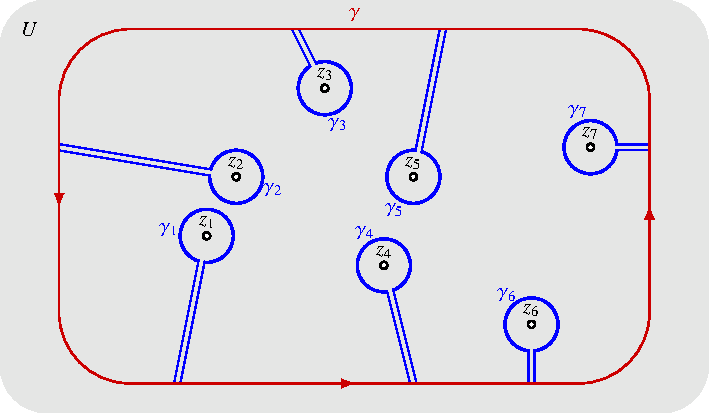
\includegraphics{chapters/030-integration/images/merohomolog.pdf}
\caption{
\label{buch:integration:homologie:fig:merohomolog}}
\end{figure}
%
In Abbildung~\ref{buch:integration:homologie:fig:merohomolog}
ist ein Gebiet $U$ mit einer einfach geschlossenen Kurve
$\gamma$ dargestellt.
Das Komplement von $U$ im Inneren der Kurve $\gamma$ besteht
aus den isolierten Punkten $z_k$.
Jeder dieser Punkte kann so mit der Kurve $\gamma$ verbunden werden,
dass sich die Verbindungen nicht schneiden.
Ausserdem wird jeder von diesen Punkten von einem kleinen Kreis $\gamma_k$
im Gegenuhrzeigersinn umlaufen.
Aus $\gamma$, den im Uhrzeigersinn durchlaufenen Kreisen $-\gamma_k$
und den Verbindungen zu $\gamma$ lässt sich ein neuer Weg zusammensetzen,
der sich in $U$ zusammenziehen lässt.
Das Wegintegral über den gesamten Weg verschwindet daher.
Die Verbindungswege zur Kurve $\gamma$ werden dabei zweimal in
entgegengesetzter Richtung durchlaufen und tragen somit nicht zum
Wegintegral bei.
Das Wegintegral einer in $U$ holomorphen Funktion über $\gamma$
ist daher gleich der Summe der Wegintegrale der Funktion
über die Kreise $\gamma_k$.

\begin{satz}
\label{buch:integration:homologie:satz:pfadpunkte}
Ist $\gamma$ eine einfach geschlossene Kurve in $U$ und besteht das Komplement
von $U$ im Inneren von $\gamma$ nur aus endlich vielen isolierten Punkten
$z_k$, $1\le k\le n$, dann gibt es einen Radius $r$ derart, dass $\gamma$
homolog zu einem Zyklus 
\[
c
=
\sum_{k=1}^n \gamma_k,
\]
wobei jedes $\gamma_k$ ein Kreis vom Radius $r$ um $z_k$ ist.
\end{satz}

\begin{proof}
Es muss nur noch der Radius $r$ berechnet werden.
Nimmt man
\[
r
=
\frac13
\min \{ |z_k-z_l|\mid 1\le k,l\le n\},
\]
dann können sich die Kreise um die Punkte $z_k$ mit Radius $r$ nicht
schneiden.
Für jeden Punkt $z_k$ ist die Umlaufzahl 
\[
\operatorname{ind}_{\gamma_k}(z_l)
=
\delta_{kl}
=
\begin{cases}
1&\qquad\text{für $k=l$}\\
0&\qquad\text{für $k\ne l$.}
\end{cases}
\]
Für den ganzen Zyklus $C$ gilt dann
\[
\operatorname{ind}_c(z_l)
=
\sum_{k=1}^n
\delta_{kl}
=
1
=
\operatorname{ind}_\gamma(z_l).
\]
Dies zeigt, dass $\gamma$ und $c$ homolog sind.
\end{proof}

%
% 54-hgruppe.tex -- Homologiegruppe
%
% (c) 2026 Prof Dr Andreas Müller
%
\subsection{Homologiegruppe}
Im Abschnitt~\ref{buch:integration:homologie:subsection:homologie}
haben wir die Homologierelation durch die Umlaufzahl um Punkte,
die ausserhalb des Definitionsgebietes liegen, definiert.
%
% fig-raender.tex
%
% (c) 2026 Prof Dr Andreas Müller
%
\begin{figure}
\centering
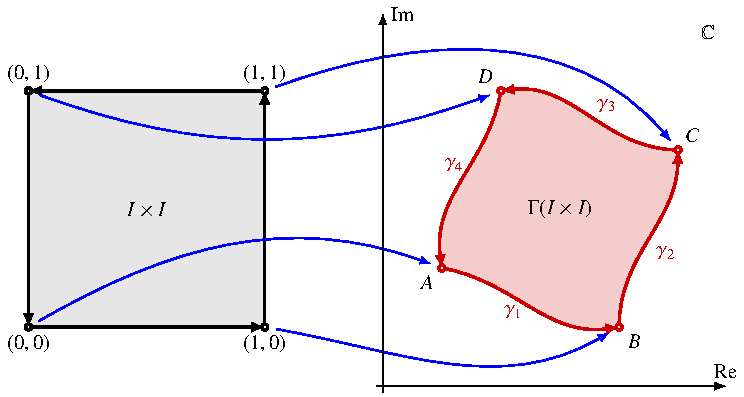
\includegraphics{chapters/030-integration/images/raender.pdf}
\caption{Zweidimensionale Kette und Rand.
\label{buch:integration:homologie:fig:raender}}
\end{figure}
%
Unter Verwendung der Homotopieeigenschaft können wir aber auch eine
algebraische Definition aufbauen.
Dazu konstruieren wir zunächst die zweidimensionalen Ketten.

\begin{definition}[Zweidimensionale Ketten]
Eine \emph{zweidimensionale Kette} ist eine formale Linearkombination
von Abbildungen 
\[
\Gamma
\colon
I\times I \to U
:
(s,t) \mapsto \Gamma(s,t)
\]
Die Menge der zweidimensionalen Ketten wird mit
\[
C_2
=
C_2(U)
=
\biggl\{
\sum_{k=1}^n c_k\Gamma_k
\;
\bigg|
\;
c_k\in\mathbb{Z}, \Gamma_k\colon I\times I\to U
\biggr\}
\]
bezeichnet.
Der \emph{Randoperator} für zweidimensionale Ketten ist die lineare
Abbildung, die einer einzelnen Abbildung $\Gamma$ die Summe
\[
\partial \Gamma
=
\gamma_1
+
\gamma_2
+
\gamma_3
+
\gamma_4
\]
zuordnet, wobei die $\gamma_k$ die Wege
\[
\renewcommand{\arraycolsep}{2pt}
\begin{array}{rlcl}
\gamma_1 &\colon I \to U&:&t\mapsto \Gamma(t,0)\\
\gamma_2 &\colon I \to U&:&t\mapsto \Gamma(1,t)\\
\gamma_3 &\colon I \to U&:&t\mapsto \Gamma(1-t,1)\\
\gamma_4 &\colon I \to U&:&t\mapsto \Gamma(0,1-t)
\end{array}
\]
sind.
\end{definition}

Die Wege $\gamma_k$ sind in
Abbildung~\ref{buch:integration:homologie:fig:raender} dargestellt.
$\gamma_1$ ist der Weg auf dem Rand von $A$ nach $B$,
$\gamma_2$ ist das Randstück von $B$ nach $C$,
$\gamma_3$ das Randstück von $C$ nach $D$ und
$\gamma_4$ das Randstück von $D$ zurück nach $A$.
Es ist offensichtlich, dass die vier Wegstücke einen geschlossenen
Weg bilden und dass daher $\partial\partial \Gamma=0$ ist.
Die Ketten $\gamma_1$ und $-\gamma_2-\gamma_3-\gamma_4$ sind homolog,
da die $\gamma_1+\gamma_2+\gamma_3+\gamma_4$ ein geschlossener
Weg ist.

Eine Abbildung $\Gamma\colon I\times I\to U$ kann man auch als
eine Homotopie zwischen den Wegen $\gamma_1$ und $\gamma
=
\gamma_4^{-1}\cdot\gamma_3^{-1}\cdot\gamma_2^{-1}$ lesen.
Auch die Zusammensetzung der roten und blauen Kurven in 
Abbildung~\ref{buch:integration:homologie:fig:residuum}
lässt sich als Rand einer Abbildung $\Gamma\colon I\times I\to U$
ansehen, die das Einheitsquadrat auf das hellrot ausgefüllte Gebiet
abbildet.
Die Tatsache, dass $\gamma$ und $-\gamma_1$ dort homolog sind, folgt
also daraus, dass sich die Kurven mithilfe einer zweidimensionalen
Kette (mit einer einzigen Abbildung $\Gamma$) ``ausfüllen'' lässt.

\begin{definition}[Ränder]
Die Menge
\[
B_1
=
B_1(U)
=
\biggl\{
\partial c
\;
\bigg|
\;
c = \sum_{k=1}^n c_k \Gamma_k\in C_2(U)
\biggr\}
=
\partial C_2(U)
\]
heisst die Menge der \emph{Ränder}.
\index{Rander@Ränder}%
\end{definition}

Die Beispiele, insbesondere auch die
Abbildung~\ref{buch:integration:homologie:fig:residuum}, zeigen,
dass homologe geschlossene Kurven sich durch den Rand einer
zweidimensionalen Kette unterscheiden.
Die Ränder $B_1$ von zweidimensionalen Ketten definieren also
eine Äquivalenzrelation von Zyklen.
Zwei Zyklen $c_1, c_2\in Z_1$ sind homolog, wenn es eine
zweidimensionale Kette $d\in C_2$ gibt derart, dass $c_1-c_2=\partial d$.
Die Zyklen unterscheiden sich daher um einen Rand.
Die Menge
\[
c+B_1(U)
=
\{
c+\partial d
\mid
d\in C_2(U)
\}
\]
besteht also aus den Zyklen, die zu $c$ homolog sind.
Diese Mengen sind die Äquivalenzklassen von Zyklen unter Äquivalenzrelation
der Homologie von Zyklen.

\begin{definition}[Homologiegruppe]
\label{buch:integration:homologie:definition:homologiegruppe}
Die Menge
\[
H_1(U)
=
Z_1(U)/B_1(U)
=
\{
c + \partial C_2
\mid
c\in Z_1(U)
\}
=
\{
c+ B_1(U)
\mid
c\in Z_1(U)
\}
\]
der Äquivalenzklassen homologer Zyklen heisst die erste
\emph{Homologiegruppe}.
\index{Homologiegruppe}%
\end{definition}

Die Definition~\ref{buch:integration:homologie:definition:homologiegruppe}
spricht von einer Gruppe, es muss also noch verifiziert
werden, dass die Addition von Zyklen ein Gruppenoperation auf $H_1(Z)$ ist.
Die Operationen werden auf den Repräsentanten in einer Äquivalenzklasse
definiert.
Daher muss gezeigt werden, dass es nicht auf die Wahl des Repräsentaten
ankommt, oder genauer, dass die Rechenoperationen mit verschiedene
Repräsentanten zu homologen Resultaten führen.
Sind $c$ und $c+\partial d$ Repräsenten der Menge der zu $c$
homologen Zyklen, dann sind ihre additiven Inversen
\(
-c
\)
und
\(
-c-\partial d
\).
Der Unterschied ist
\[
-c
-(
-c-\partial d
)
=
\partial d \in B_1.
\]
Die beiden Repräsentaten von $-c$ sind also homolog und repräsentieren
die selbe Äquivalenzklasse.
Für die Addition betrachten wir Repräsentanten $a$ und $a+\partial d_a$
bzw.~$b$ und $b+\partial d_b$.
Die Summen unterscheiden sich um
\[
(a+b)-(a+\partial d_a+b+\partial d_b)
=
-\partial(d_a+d_b)
\in
B_1(U),
\]
wobei die letzte Umformung aus der Linearität des Randoperators folgt.
Die beiden Repräsentanten der Summe $a+b$ sind daher homolog.

Ränder sind zusammenziehbare Kurven, das Wegintegral über einen
Rand verschwindet daher immer.
Dies zeigt erneut, dass Wegintegrale über homologe Zyklen gleich sind.
Das Wegintegral einer Funktion $f$ definiert also eine lineare Abbildung
von Klassen homologer Zyklen.

\begin{satz}
Die Abbildung
\[
\oint f(z)\,dz
\colon
H_1(U) \to \mathbb{C}
:
c
\mapsto
\oint_c f(z)\,dz
\]
ist eine lineare Abbildung.
\end{satz}

%
% 55-dimension.tex -- Homologie in höheren Dimensionen
%
% (c) 2026 Prof Dr Andreas Müller
%
\subsection{Homologie in anderen Dimensionen}
Die Homologiegruppe $H_1(U)$ von $U$ gibt Information über die 
Zusammenziehbarkeit von geschlossenen Kurven.
Damit lässt sich aber noch nicht entscheiden, ob $U$ aus verschiedenen,
nicht verbundenen Komponenten besteht.
Die Homologiegruppe $H_0$ löst dieses Problem.
Im dreidmensionalen Raum $U=\mathbb{R}^3\setminus\{0\}$ ohne den
Nullpunkt ist jede Kurve zusammeziehbar, die Homologiegruppe $H_1$
kann also das Fehlen des Nullpunktes nicht detektieren.
Dazu brauchte es die höhere Homologiegruppe $H_2(U)$.

%
% H_0: die Zusammenhangskomponenten von U
%
\subsubsection{$H_0(U)$: Die Zusammenhangskomponenten von $U$}
Eine zur Konstruktion der Homologiegruppe $H_1(U)$ analoge Konstruktion
kann auch eine Dimension tiefer durchgeführt werden.
In Definition~\ref{buch:integration:homologie:definition:randoperator}
wurden bereits die $0$-Ketten definiert und es wurde illustriert,
wie der Randoperator aus einer $1$-Kette eine $0$-Kette macht.
Die Menge
\[
B_0(U)
=
\{
\partial c
\mid
c\in C_1(U)
\}
\]
wird erzeugt von Paaren von Punkten, die durch eine Kurve 
verbunden sind.
Wir sagen wieder, zwei $0$-Ketten sind homolog, wenn sie sich
um den Rand einer $1$-Kette unterscheiden.
Damit lässt sich wieder eine Gruppe
\[
H_0(U)
=
C_0(U) / B_0(U)
=
c + B_0(U)
=
\{
c + \partial d
\mid
d\in C_1(U)
\}
\]
konstruieren.
Sie wird erzeugt von homologen Punkten.

\begin{satz}[Wegzusammenhang]
Wenn zu zwei beliebigen Punkten $P_1,P_2\in U$ die $0$-Kette
$P_2-P_1$ ein Rand einer $1$-Kette $c$ ist, dann gibt es einen Weg
zwischen $P_1$ und $P_2$.
Eine Teilmenge $U$ von $\mathbb{C}$ ist genau dann wegzusammenhängend,
\index{wegzusammenhangend@wegzusammenhängend}%
wenn es eine $1$-Kette $c \in C_1(U)$ gibt mit
$\partial c=P_2-P_1$.
\end{satz}

\begin{proof}
Wenn es einen Weg $\gamma$ zwischen $P_1$ und $P_2$ gibt, z.~B.~weil $U$
wegzusammenhängend ist, dann hat die
$1$-Kette $c=\gamma$ den verlangten Rand $\partial c = P_2-P_1$.

Wenn es eine $1$-Kette
\[
c
=
\sum_k
c_k\gamma_k
\]
mit $\partial c = P_2-P_1$ gibt, dann lassen sich die $\gamma_k$ zu einem
Weg zusammensetzen, der in $P_1$ beginnt und in $P_2$ endet.
Nicht unbeding alle Wege der Kette werden verwendet.
Einige Wege in der Kette bilden geschlossene Wege, die ignoriert
werden können.
Die Verkettung der Wege ist ein möglicherweise nicht differenzierbarer
Weg, somit liegen $P_1$ und $P_2$ in der gleichen Wegzusammenhangskomponente.
\end{proof}

Die Homologiegruppe $H_0(U)$ wird erzeugt von den
Zusammenhangskomponenten.
Natürlich enthält auch $H_1(U)$ Information über die
Zusammenhangskomponenten, da geschlossene Wege jeweils in einer
einzelnen Zusammenhangskomponente enthalten sind und daher
Wege in verschiedenen Zusammenhangskomponenten nicht homolog sein
können.

%
% Höhere Homologiegruppen
%
\subsubsection{Höhere Homologiegruppen}
Die Konstruktionen, die zur Homologiegruppe $H_1$ geführt haben,
lassen sich in jeder beliebigen Dimension durchführen.
Im folgenden sei daher $k>1$ eine natürliche Zahl.
Eine $k$-dimensionale Kette ist eine formale Linearkombination
von Abbildungen des $k$-dimensionalen Einheitswürfels
\[
\Gamma
\colon
I^k
\to
U
:
(t_1,\dots,t_k)
\mapsto
\Gamma(t_1,\dots,t_k).
\]
Die $(k-1)$-dimensionalen Seitenflächen des Würfels sind Abbildungen
der Form
\begin{align*}
\Gamma_i^0
&
\colon I^{k-1}\to U
:
(s_1,\dots,s_{k-1})
\mapsto
\Gamma(s_1,\dots,s_{i-1},0,s_{i},\dots,s_{k-1})
\intertext{und}
\Gamma_i^1
&
\colon I^{k-1}\to U
:
(s_1,\dots,s_{k-1})
\mapsto
\Gamma(s_1,\dots,s_{i-1},1,s_{i},\dots,s_{k-1})
\end{align*}
für $i=1,\dots,k-1$.
Der Randoperator ist wieder die lineare Abbildung, die auf $\Gamma$
als eine Linearkombination von $\Gamma^0_i$ und $\Gamma^1_i$ 
mit Koeffizienten $\pm1$.

Ein $k$-dimensionaler Zyklus ist eine $k$-dimensionale Kette $c$ mit
der Eigenschaft $\partial c=0$.
Die Menge der $k$-dimensionalen Zyklen wird mit
\[
Z_k
=
Z_k(U)
=
\{
c\in C_k(U)
\mid
\partial c=0
\}
\]
bezeichnet.

Der Randoperator auf $C_{k+1}$ liefert zu einem $(k+1)$-dimensionalen
Würfel die Oberfläche des Würfels, bestehend aus $k$-dimensionalen
Würfeln.
Die Menge der $k$-dimensionalen Ränder ist
\[
B_k
=
B_k(U)
=
\partial C_k(U).
\]
Zwei $k$-dimensionale Zyklen heissen homolog, wenn sie sich um
einen $k$-dimensionalen Rand unterscheiden, wir können daher auch
eine $k$-dimensionale Homologiegruppe
\[
H_k(U)
=
Z_k(U) / B_k(U)
=
\{
c + B_k(U)
\mid
c\in Z_k(U)
\}
\]
konstruieren.

%
% Homologiegruppen und Homotopie
%
\subsubsection{Homologiegruppen und Homotopie}
Man kann jeweils eines der Argument einer Abbildung $\Gamma$
eines $k$-dimensionalen Würfels als den Homotopieparameter
betrachten.
Die Abbildung wird dann als eine Homotopie zwischen zwei
$(k-1)$-dimensionalen Würfeln interpretiert.
Die Homologiegruppe betrachtet daher homotope $(k-1)$-dimensionale
Zyklen als homolog, wenn sie homotop sind.

Die Menge $U=\mathbb{R}^3$ ist zusammenziehbar, jeder Abbildung $\Gamma$
ist daher homotop zur konstanten Abbildung in den Nullpunkt.
Daher sind alle $k$-dimensionalen Zyklen auch Ränder und alle
Elemente in $Z_k(U)$ sind homolog.
Die Homologiegruppen sind daher $H_k(\mathbb{R})=\{0\}$.

%
% Homologiegruppen und Löcher
%
\subsubsection{Homologiegruppen und ``Löcher''}
Die Homologiegruppe $H_1(U)$ erkennt die Löcher in einem zweidimensionalen
Gebiet $U$.
Die Homologiegruppen $H_k$ mit $k>1$ erkennen höherdimensionale ``Löcher''.

Als Beispiel untersuchen wir die die Menge $U=\mathbb{R}\setminus \{0\}$.
Die Abbildung
\[
\Gamma
\colon
I^3
\to
\mathbb{R}^3
:
(t_1,t_2,t_3)
\mapsto
(
t_1-{\textstyle\frac12},
t_2-{\textstyle\frac12},
t_3-{\textstyle\frac12}
)
\]
ist keine Abbildung in $U$, da der Punkt $(\frac12,\frac12,\frac12)$ auf
den Nullpunkt abgebildet wird, der nicht in $U$ ist.
Der Randoperator liefert aber eine Linearkombination der Randquadrate,
die in $U$ enthalten sind.
Sie bilden einen Zyklus, da die Ränder der einzelnen Quadrate alle
in beiden Richtungen durchlaufen werden.
Dieser Zyklus ist also nicht in $B_2(U)$ enthalten.
Jede Abbildung von $I^3\to \mathbb{R}^3$, die den Nullpunkt trifft,
hat als Rand einen Zyklus in $U$, der nicht ein Rand sein kann.
Somit gibt es in der Homologiegruppe $H_2$ genau einen Zyklus, der
nicht homolog zur konstanten Abbildung ist.
Somit ist $H_2(U)=\mathbb{Z}$.
Die Homologiegruppe $H_2(U)$ hat also das Loch im Nullpunkt erkannt.

